\documentclass[tikz,border=15pt]{standalone}
\usepackage{amsmath,amssymb}
\usetikzlibrary{decorations.pathreplacing, calc, shadows, arrows.meta}
\usepackage[T1]{fontenc}
\usepackage[utf8]{inputenc}
\usepackage{newpxtext,newpxmath}
\usepackage{sectsty}
% Define the color palette
\definecolor{accent}{RGB}{20, 80, 180}       % Blue for Identity/Info
\definecolor{softaccent}{RGB}{230, 240, 255} 
\definecolor{parity}{RGB}{210, 80, 30}       % Orange for Parity/A
\definecolor{softparity}{RGB}{255, 235, 225} 
\definecolor{transform}{RGB}{120, 40, 160}   % Purple for Matrix U
\definecolor{softtransform}{RGB}{245, 235, 255}

\newcommand{\F}{\mathbb F}
\newcommand{\vect}[1]{\mathbf{#1}}

\begin{document}
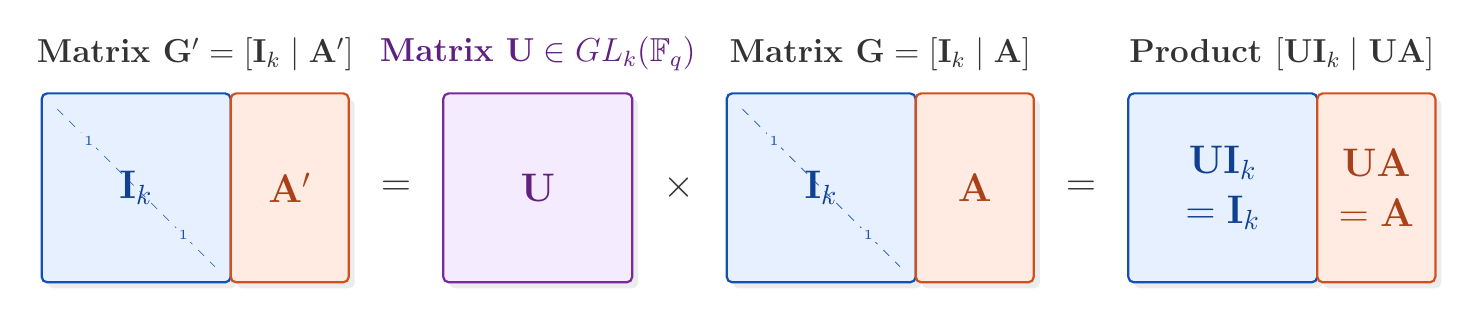
\begin{tikzpicture}[
	>=Stealth,
	font=\sffamily,
	% Styles for the matrix blocks
	infoblock/.style={draw=accent, thick, fill=softaccent, rounded corners=2pt, drop shadow={opacity=0.15}},
	parityblock/.style={draw=parity, thick, fill=softparity, rounded corners=2pt, drop shadow={opacity=0.15}},
	transformblock/.style={draw=transform, thick, fill=softtransform, rounded corners=2pt, drop shadow={opacity=0.15}},
	% Styles for text and logic nodes
	labeltext/.style={text=black!80},
	mathsym/.style={font=\Large\bfseries, text=black!80},
	logicnode/.style={fill=white, draw=black!30, thick, rounded corners=3pt, font=\small, align=center, inner sep=6pt, drop shadow={opacity=0.1}}
	]
	
	% NOTE: Height is 2.4 (from -1.2 to 1.2). 
	% To make k x k blocks square, their width is strictly set to 2.4.
	
	% ==========================================
	% LHS: MATRIX G'
	% ==========================================
	% I_k is now a 2.4 x 2.4 square
	\draw[infoblock] (0, -1.2) rectangle (2.4, 1.2);
	\node[mathsym, text=accent!80!black] at (1.2, 0) {$\vect{I}_k$};
	% Faint 1s across the exact diagonal
	\draw[accent, very thin, dashed] (0.2, 1.0) -- (2.2, -1.0);
	\node[text=accent, font=\tiny, fill=softaccent, inner sep=1pt] at (0.6, 0.6) {$1$};
	\node[text=accent, font=\tiny, fill=softaccent, inner sep=1pt] at (1.8, -0.6) {$1$};
	
	\draw[parityblock] (2.4, -1.2) rectangle (3.9, 1.2);
	\node[mathsym, text=parity!80!black] at (3.15, 0) {$\vect{A}'$};
	
	\node[labeltext, font=\large\bfseries] at (1.95, 1.7) {Matrix $\vect{G}'=[\vect{I}_k \mid \vect{A}']$};
%	\node[labeltext, font=\scriptsize] at (1.95, 2.1) {$[I_k \mid A']$};
	
	% Equals sign
	\node[mathsym] at (4.5, 0) {$=$};
	
	% ==========================================
	% RHS PART 1: MATRIX U
	% ==========================================
	% U is k x k, so it is also a 2.4 x 2.4 square
	\draw[transformblock] (5.1, -1.2) rectangle (7.5, 1.2);
	\node[mathsym, text=transform!80!black] at (6.3, 0) {$\vect{U}$};
	
	\node[labeltext, font=\large\bfseries, text=transform!80!black] at (6.3, 1.7) {Matrix $\vect{U}\in GL_k(\F_q)$};
%	\node[labeltext, font=\scriptsize, text=transform] at (6.3, 2.1) {Invertible $\in GL_k(\F_q)$};
	
	% Multiplication sign
	\node[mathsym] at (8.1, 0) {$\times$};
	
	% ==========================================
	% RHS PART 2: MATRIX G
	% =================6=========================
	% I_k is a 2.4 x 2.4 square
	\draw[infoblock] (8.7, -1.2) rectangle (11.1, 1.2);
	\node[mathsym, text=accent!80!black] at (9.9, 0) {$\vect{I}_k$};
	% Faint 1s
	\draw[accent, very thin, dashed] (8.9, 1.0) -- (10.9, -1.0);
	\node[text=accent, font=\tiny, fill=softaccent, inner sep=1pt] at (9.3, 0.6) {$1$};
	\node[text=accent, font=\tiny, fill=softaccent, inner sep=1pt] at (10.5, -0.6) {$1$};
	
	\draw[parityblock] (11.1, -1.2) rectangle (12.6, 1.2);
	\node[mathsym, text=parity!80!black] at (11.85, 0) {$\vect{A}$};
	
	\node[labeltext, font=\large\bfseries] at (10.65, 1.7) {Matrix $\vect{G}=[\vect{I}_k \mid \vect{A}]$};
%	\node[labeltext, font=\scriptsize] at (10.65, 2.1) {$[I_k \mid A]$};
	
	% Equals sign
	\node[mathsym] at (13.2, 0) {$=$};
	
	% ==========================================
	% RHS PRODUCT: U * G
	% ==========================================
	% UI_k block (2.4 x 2.4)
	\draw[infoblock] (13.8, -1.2) rectangle (16.2, 1.2);
	\node[mathsym, text=accent!80!black, align=center] at (15.0, 0) {$\vect{U} \vect{I}_k$\\ $=\vect{I}_k$};
	
	% UA block
	\draw[parityblock] (16.2, -1.2) rectangle (17.7, 1.2);
	\node[mathsym, text=parity!80!black, align=center] at (16.95, 0) {$\vect{U} \vect{A}$\\ $=\vect{A}$};
	
	\node[labeltext, font=\large\bfseries] at (15.75, 1.7) {Product $[\vect{U} \vect{I}_k \mid \vect{U} \vect{A}]$};
%	\node[labeltext, font=\scriptsize] at (15.75, 2.1) {$[U I_k \mid U A]$};
	
%	% ==========================================
%	% LOGICAL DEDUCTION ARROWS
%	% ==========================================
%	
%	% Step 1: Equating Identity Blocks (Underneath)
%	\draw[<->, accent, thick, dashed] (1.2, -1.4) to[out=270, in=270, looseness=0.35] 
%	node[midway, logicnode] {
%		\color{accent!80!black}\textbf{Step 1: Equating the Identity blocks}\\[1ex]
%		$I_k = U I_k \implies \mathbf{U = I_k}$
%	} (15.0, -1.4);
%	
%	% Step 2: Equating Parity Blocks (Overhead)
%	\draw[<->, parity, thick, dashed] (3.15, 2.5) to[out=90, in=90, looseness=0.3] 
%	node[midway, logicnode] {
%		\color{parity!80!black}\textbf{Step 2: Equating the Parity blocks}\\[1ex]
%		$A' = U A \quad \xrightarrow{\text{Substitute } U=I_k} \quad I_k A \implies \mathbf{A' = A}$
%	} (16.95, 2.5);
%	
%	% ==========================================
%	% CONCLUSION BOX
%	% ==========================================
%	\node[logicnode, inner sep=10pt, draw=transform!80!black] at (8.85, -4.8) {
%		\Large\bfseries Conclusion: $G' = G$ \\[1ex]
%		\normalsize\normalfont The systematic generator matrix for a given set of information coordinates is \textbf{strictly unique}.
%	};
	
\end{tikzpicture}
\end{document}